\chapter{Arhitektura i dizajn sustava}


		    \textit{ Za izradu naše web aplikacije odlučili smo se za trenutno veoma popularnu MVC (eng. Model-View-Controller)  arhitekturu. Kao što ime sugerira, ima tri glavna dijela. Tradicionalni obrazac softverskog dizajna funkcionira u obrascu "ulaz - proces - izlaz", dok MVC djeluje kao "kontroler - model - pogled". Ukratko ćemo opisati svaki od ova 3 dijela: }
		
		  \begin{packed_item}
	        \item 	\textit{Model - ova klasa koristi se za provođenje logike provjere valjanosti i poslovnih pravila podataka. Nije usko vezan uz korisničko sučelje, što znači da možemo tu klasu iskoristiti i upotrijebiti u različitim vrstama aplikacija poput aplikacija radne površine ili mobilne aplikacije.    }
		    \item 	\textit{View - odgovoran za prikazivanje svih ili dijela podataka korisniku, obavještava upravljač te ponekad ažurira model slanjem odgovarajućih poruka}
		    \item 	\textit{Controller - Upravljač je između modela i elementa prikaza. Sluša sve incidente i radnje pokrenute u prikazu i izvodi odgovarajući odgovor na događaje. Korisnik obično djeluje s prikazom i izvodi neke radnje na zaslonu. Zahtjev se generira iz prikaza kojim upravlja upravljač. To čini upravljač odgovornim za rukovanje http zahtjevom.  }	
		\end{packed_item}

	        \textit {     MVC je popularan jer izolira aplikacijsku logiku iz sloja korisničkog sučelja i podržava odvajanje problema. Upravljač prima sve zahtjeve vezane za aplikaciju, a zatim radi s modelom kako bi pripremio sve podatke potrebne za prikaz. Prikaz tada koristi podatke pripremljene od strane upravljača za generiranje konačnog prezentiranog odgovora. Također, često se koristi zbog velikog broja beneficija kao što su brži razvojni proces (jedan programer može raditi na prikazu, dok drugi može raditi na kontroleru za stvaranje poslovne logike web aplikacije.), podrška za asinkronu tehniku (podržava i JavaScript okvir, što znači da aplikacije mogu raditi i s PDF-ovima), mogućnošću većeg broja prikaza (View-ova) te mnogih drugih.}
		

		
	\newpage
				
	\section{Baza podataka}
	
	\textit Za potrebe našeg sustava koristit ćemo SQL relacijsku bazu podataka. Odlučili smo se za tu bazu podataka budući da se relacijska struktura u velikoj mjeri podudara s percepcijom događaja stvarnog svijeta. Relacijska baza podataka sastoji se od skupa povezanih tablica odnosno relacija. Svaka se relacija sastoji od naziva te skupa atributa koji su u sastavu te tablice. Podaci su pohranjeni zajedno na način neovisan o programima koji ih koriste, uz isključenje bespotrebne zalihosti (redundancije). Zadaća baze podataka je brza i jednostavna pohrana, izmjena i dohvat podataka koji će se dalje obrađivati. 
	Baza podataka ove aplikacije sastoji se od sljedećih entiteta: MuseumObjects, Role, User, Statistics.
	
	\subsection{Opis tablica}
	
	\textit MuseumObject  - ovaj entitet sadrži sve informacije o muzejskom objektu. Sadrži atribute: id, name, description, imageName, tag, audioName i statisticsId. 
	Ovaj entitet u vezi je One-to-One s Statistics preko statisticsId.
	
	\begin{longtabu} to \textwidth {|X[6, l]|X[6, l]|X[20, l]|}
		
		\hline \multicolumn{3}{|c|}{\textbf{MuseumObject}}	 \\[3pt] \hline
		\endfirsthead
		
		\hline \multicolumn{3}{|c|}{\textbf{MuseumObject}}	 \\[3pt] \hline
		\endhead
		
		\hline 
		\endlastfoot
		
		\cellcolor{LightGreen}id & INT	&  	jedinstven identifikator muzejskog objekta	\\ \hline
		name	& VARCHAR(255) &  naziv muzejskog objekta 	\\ \hline 
		description & VARCHAR(1600) &  opis muzejskog objekta \\ \hline 
		imageName & VARCHAR(255)	&  naziv slike		\\ \hline 
		tag & VARCHAR(255)	&  oznaka muzejskog objekta		\\ \hline
		audioName & VARCHAR(255)	&  naziv zvučnog zapisa		\\ \hline
		\cellcolor{LightBlue} statisticsId & INT	&  jedinstveni identifikator statistike		\\ \hline
	\end{longtabu}

	\textit Statistics - ovaj entitet sadrži sve informacije o statistici aplikacije. Sadrži atribute: id, pageTraffic, time i audioStarted.
	
	\begin{longtabu} to \textwidth {|X[6, l]|X[6, l]|X[20, l]|}
		
		\hline \multicolumn{3}{|c|}{\textbf{Statistics}}	 \\[3pt] \hline
		\endfirsthead
		
		\hline \multicolumn{3}{|c|}{\textbf{Statistics}}	 \\[3pt] \hline
		\endhead
		
		\hline 
		\endlastfoot
		
		\cellcolor{LightGreen}id & INT	&  jedinstven identifikator statistike 	\\ \hline
		pageTraffic & INT 	&  	posjećenost stranice	\\ \hline 
		time & INT 	&  	vrijeme provedeno na stranici	\\ \hline 
		audioStarted & INT 	&  	broj pokretanja zvučnog zapisa	\\ \hline 		
	\end{longtabu}
	
	\newpage
	
	\textit User - ovaj entitet sadrži sve informacije o korisnicima aplikacije. Sadrži atribute: id, username, firstName, lastName, email, passwordHash, role, currentlyActive i accConfirmed. Ovaj entitet u vezi je Many-to-One s Role preko roleId.
	
	\begin{longtabu} to \textwidth {|X[6, l]|X[6, l]|X[20, l]|}
		
		\hline \multicolumn{3}{|c|}{\textbf{User}}	 \\[3pt] \hline
		\endfirsthead
		
		\hline \multicolumn{3}{|c|}{\textbf{User}}	 \\[3pt] \hline
		\endhead
		
		\hline 
		\endlastfoot
		
		\cellcolor{LightGreen}id & INT	&  jedinstven identifikator korisnika 	\\ \hline
		username	& VARCHAR(255) & korisničko ime  	\\ \hline 
		firstName & VARCHAR(255)	&  	ime korisnika	\\ \hline
		lastName & VARCHAR(255)	&  prezime korisnika		\\ \hline
		email & VARCHAR(255) &  email adresa korisnika \\ \hline 
		passwordHash & VARCHAR(255) 	&  	hash lozinke	\\ \hline 
		\cellcolor{LightBlue} roleId & INT	&  	uloga korisnika	\\ \hline	
		currentlyActive & BOOLEAN	&  	trenutno aktivan	\\ \hline	
		accConfirmed & BOOLEAN	&  	korisnički račun potvrđen	\\ \hline		
	\end{longtabu}

	\textit Role - ovaj entitet sadrži informacije o mogućim ulogama korisnika ove aplikacije. Sadrži atribute: id i name.
	
	\begin{longtabu} to \textwidth {|X[6, l]|X[6, l]|X[20, l]|}
		
		\hline \multicolumn{3}{|c|}{\textbf{Role}}	 \\[3pt] \hline
		\endfirsthead
		
		\hline \multicolumn{3}{|c|}{\textbf{Role}}	 \\[3pt] \hline
		\endhead
		
		\hline 
		\endlastfoot
		
		\cellcolor{LightGreen}id & INT	&  	jedinstven identifikator uloge 	\\ \hline
		name	& VARCHAR(255) &  naziv uloge 	\\ \hline 		
		
	\end{longtabu}
	
	
			
			\newpage
			\subsection{Dijagram baze podataka}
				
				\begin{figure}[H]
					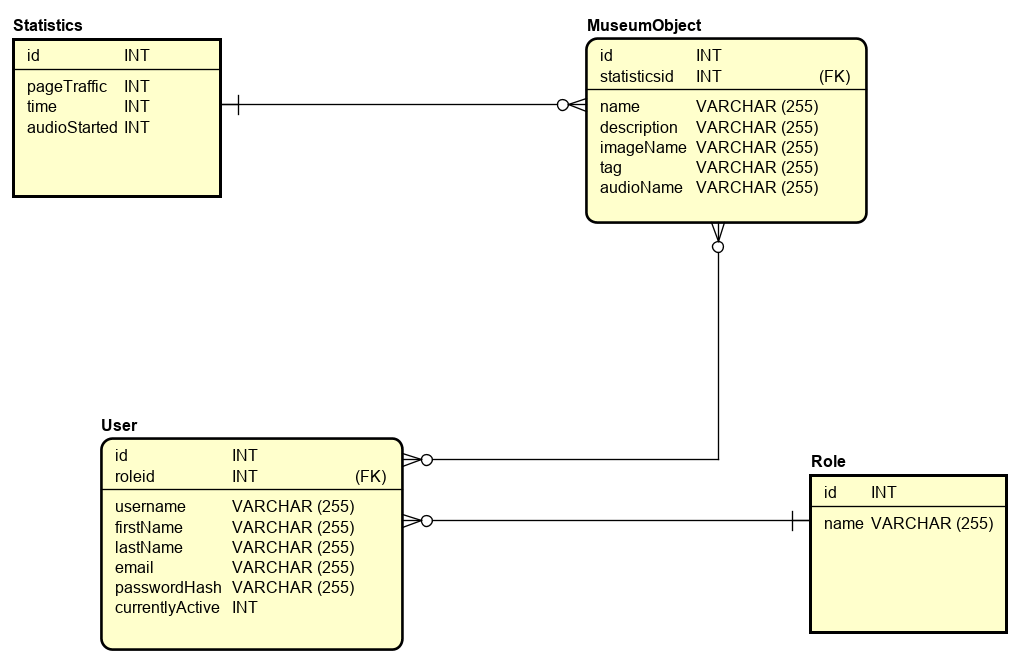
\includegraphics[scale=0.6]{slike/ER_Dijagram.png}
					\centering
					\caption{E-R dijagram baze podataka}
					\label{fig:promjene}
				\end{figure}
			
			\eject
			
			
		\section{Dijagram razreda}
		
			\begin{figure}[H]
				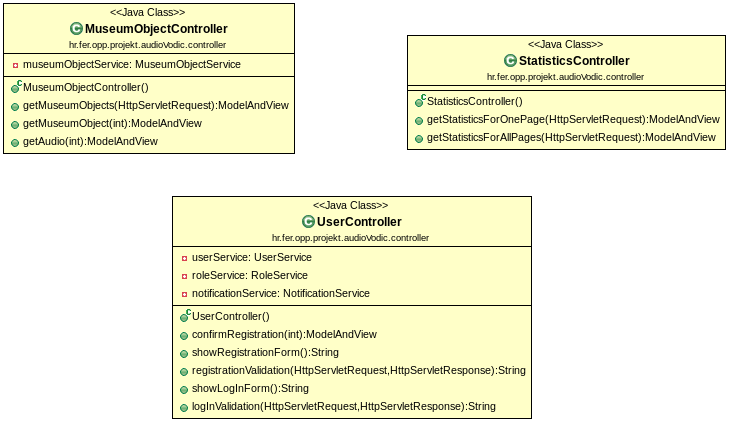
\includegraphics[scale=0.6]{slike/Controller.png}
				\centering
				\caption{ Dijagram razreda - dio Controllers}
				\label{fig:promjene}
			\end{figure}
		
			\begin{figure}[H]
				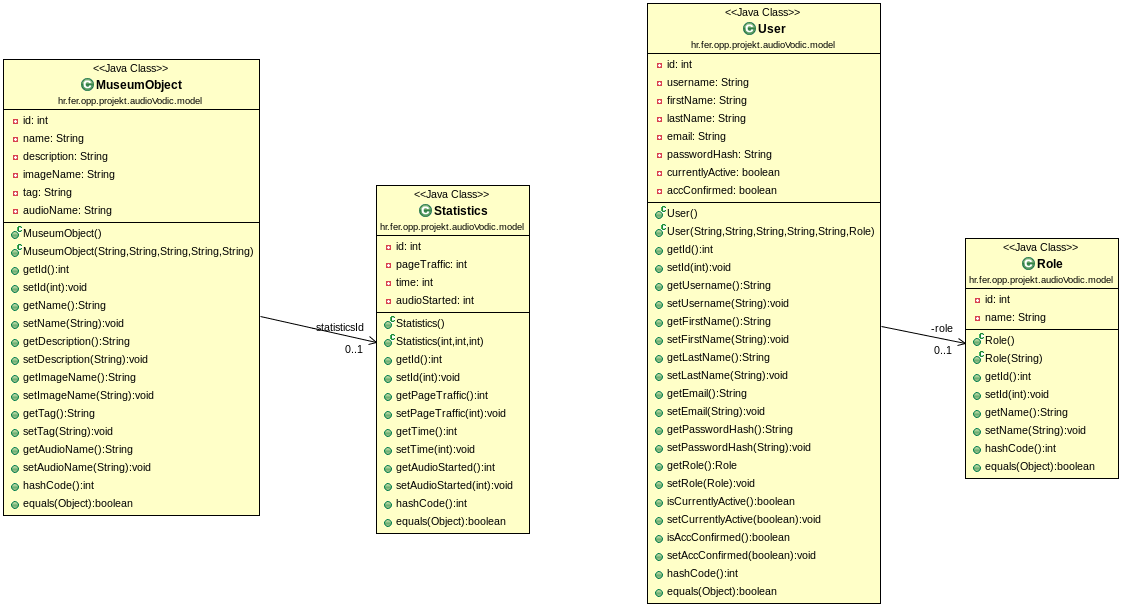
\includegraphics[scale=0.4]{slike/Models.png}
				\centering
				\caption{Dijagram razreda - dio Models}
				\label{fig:promjene}
			\end{figure}
			
		
		
		
		
		
		
		
		
		
		
		\section{Dijagram stanja}
		
			\begin{figure}[H]
				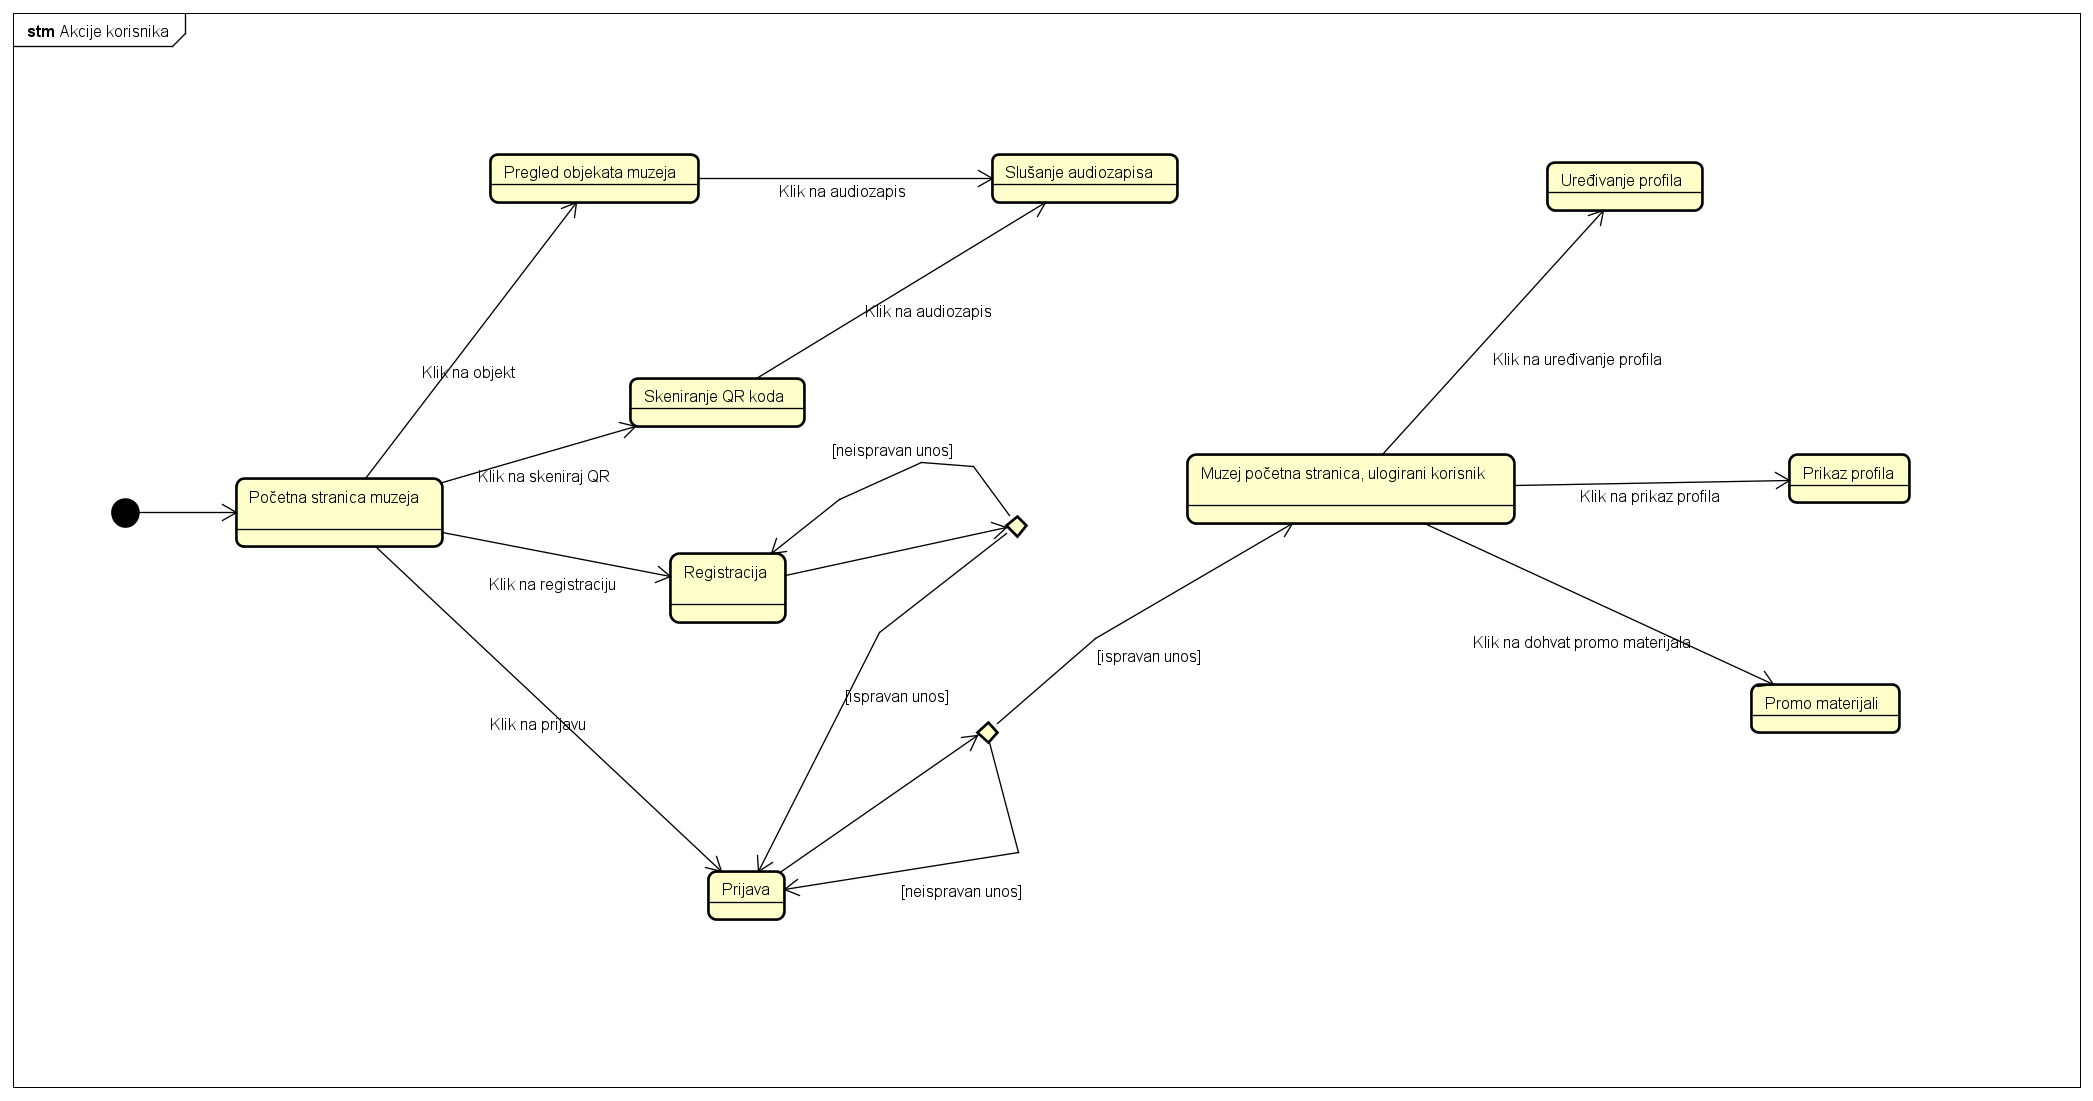
\includegraphics[scale=0.32]{slike/Dijagramstanja.png}
				\centering
				\caption{Dijagram stanja}
				\label{fig:promjene}
			\end{figure}
		
		
		\textit Dijagram stanja je ponašajni, dinamički dijagram koji prikazuje ponašanje sustava, tojest aktivnost i prijelaz između stanja uzrokovan vanjskim događajima. Na slici je dijagram stanja za korisnike na stranici muzeja, prikazuje sva moguća stanja neregistriranih i registriranih korisnika. Neregistrirani korisnik može proučavati muzejske objekte, slušati videozapise i skenirati QR kod. Registrirani korisnik uz sve to može pregledati i urediti svoj osobni profil te dohvatiti promo materijale.
		
		
		\eject 
		
		\section{Dijagram aktivnosti}
		
    		\begin{figure}[H]
				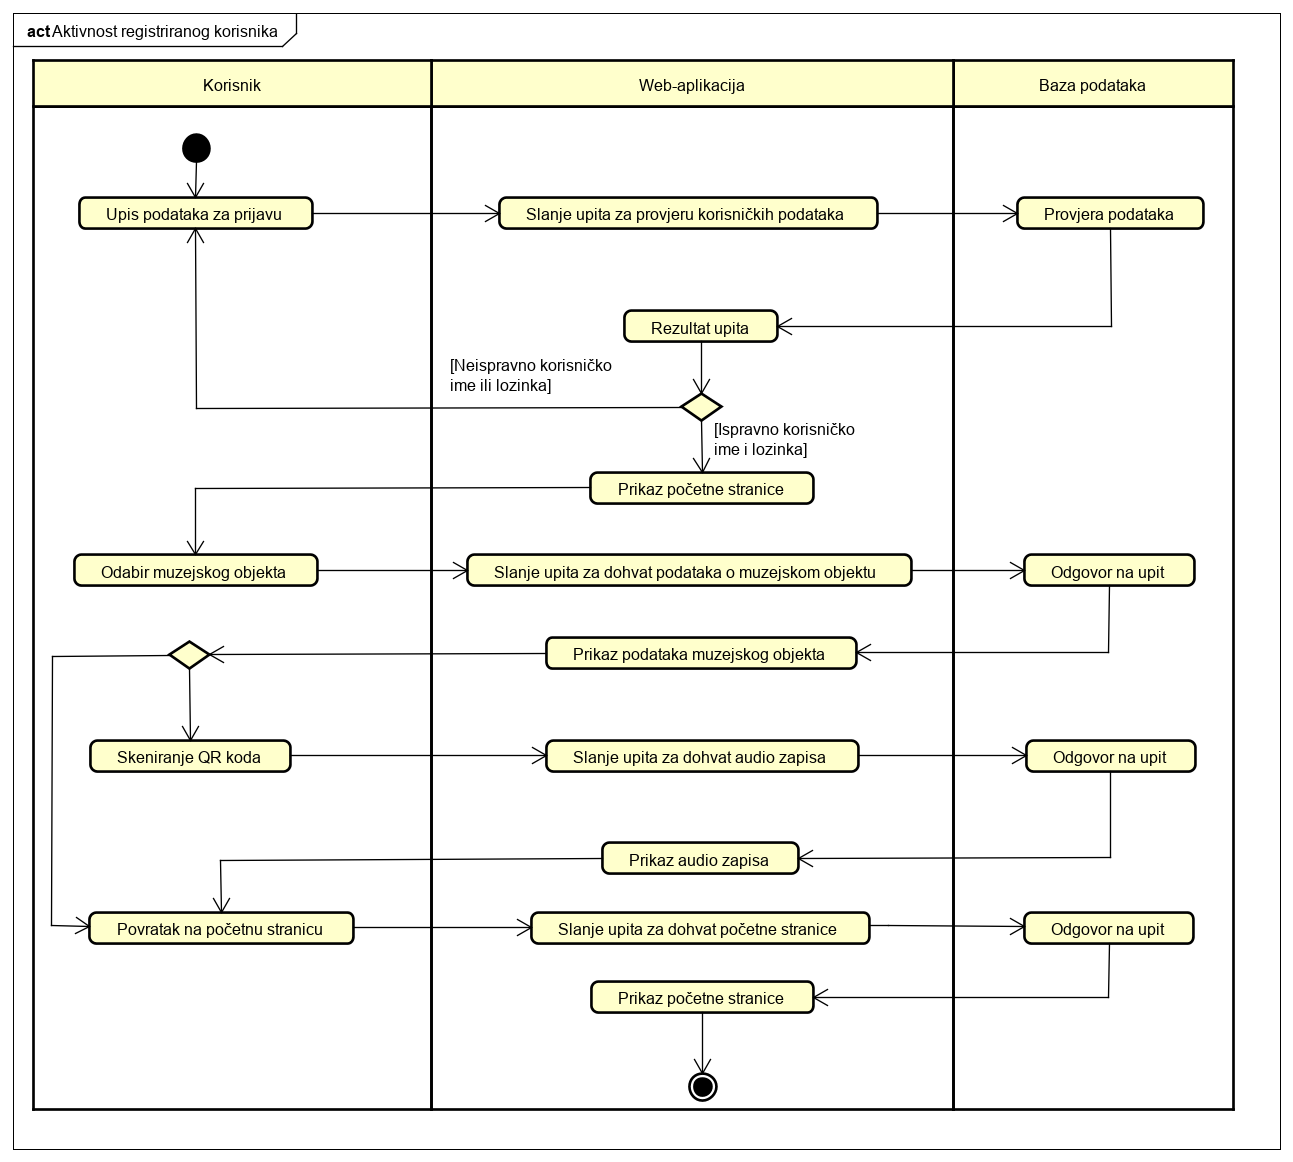
\includegraphics[scale=0.5]{slike/dijagram_aktivnosti.png}
				\centering
				\caption{Dijagram aktivnosti}
				\label{fig:promjene}
			\end{figure}
		
		\textit Dijagram aktivnosti ponašajni je i dinamički dijagram te je specijalni slučaj dijagrama stanja u kojem su sva stanja akcije, a promjena je inicirana završetkom akcije u izvornom stanju. Koristi se za prikaz modela toka upravljanja ili toka podataka. Slika prikazuje dijagram aktivnosti registriranog korisnika koji želi proučiti muzejski objekt. Korisnik se prijavljuje u sustav i bira muzejski izložak s početne stranice. Web-aplikacija iz baze uzima podatke o izlošku koje prenosi korisniku. Korisnik može pokrenuti audio zapis s informacijama o muzejskom objektu ili se vratiti na početnu stranicu te nastaviti pregled muzejskih objekata.
		
		\eject
		\section{Dijagram komponenti}
		    \begin{figure}[H]
				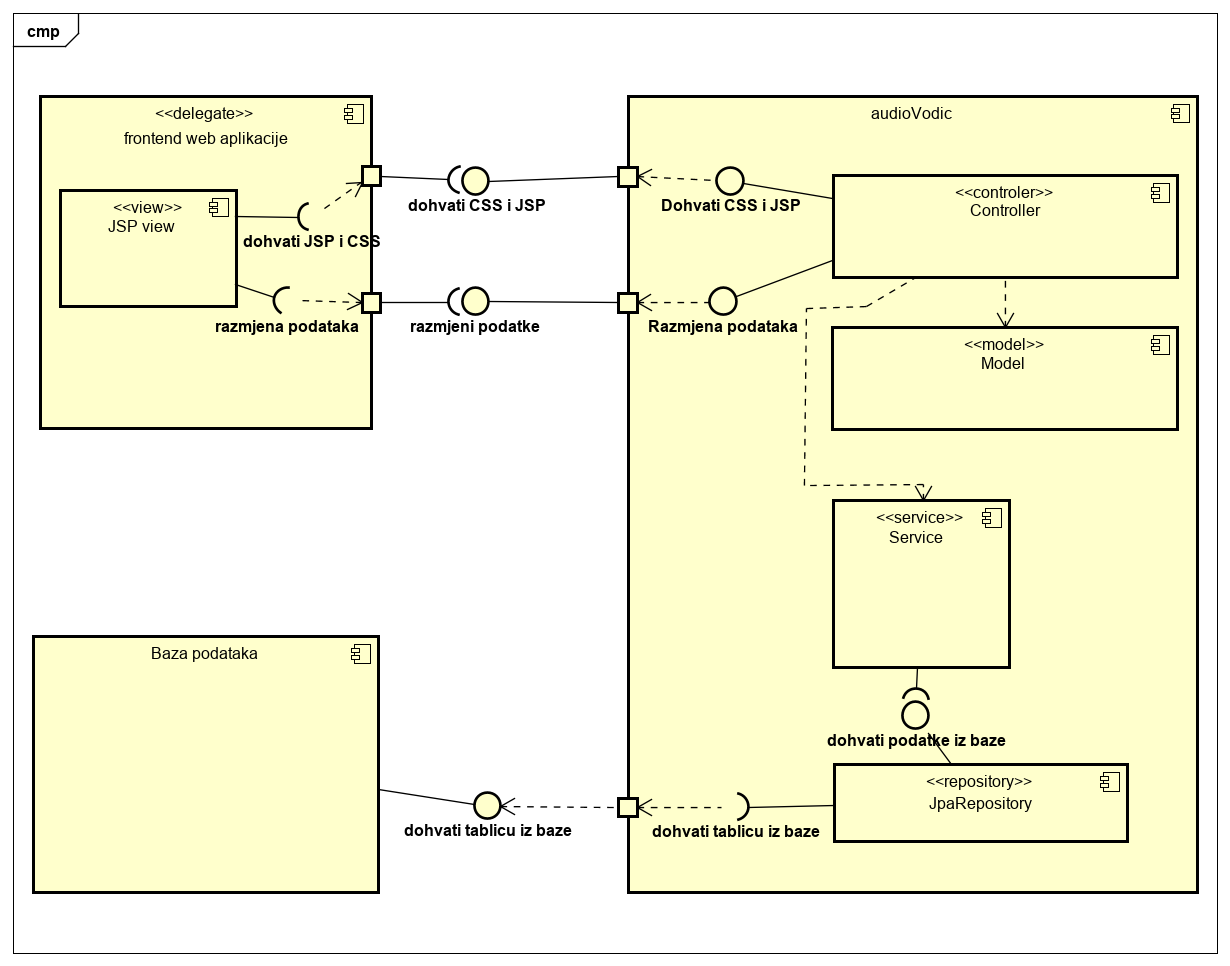
\includegraphics[scale=0.5]{slike/dijagram_komponenti.png}
				\centering
				\caption{Dijagram komponenti}
				\label{fig:promjene}
			\end{figure}
		
		\textit Dijagram komponenti je dijagram koji se odnosi na implementaciju sustava i prikazuje međusobnu zavisnost programskih komponenti, interne strukture te odnos prema okolini. Njegova je namjena vizualizacija organizacije i odnosa među komponentama sustava. Slika dijagrama komponenti predočuje kako se sustavu pristupa preko dva različita sučelja. Prvo se sučelje odnosi na dohvat CSS i JSP datoteka koje se nalaze u frontent dijelu aplikacije. Drugo sučelje služi za razmjenu podataka. JpaRepository zadužen je za dohvaćanje tablica iz baze podataka pomoću SQL upita.